\section{Introduction}
\IEEEPARstart{T}{ank} trucks hold a vital role in road transportation, with about 80\% of the nation's liquid hazardous materials being transported by this means\cite{200Accidents}. However, the issue of tank truck rollovers has been a long-standing traffic safety hazard, causing significant accidents in cities such as Wenling, Ya'an, and Dongying\cite{WenlingAccidents}. These accidents represent a substantial threat to public safety and property. Tank trucks, making up 18\% of commercial trucks, are involved in over 30\% of rollover accidents\cite{ChinaRailway}. The root causes include their high center of gravity, partial loading\cite{GB18564-1,TSGR0005-2011}, and the vehicle-liquid coupling characteristics, which greatly reduce their rollover stability. Under improper operation or extreme conditions, these trucks are prone to rollovers, leading to severe secondary accidents such as fires, explosions, and environmental pollution. Hence, the study of tank truck rollover prevention is of significant real-world relevance.

The prevention of tank truck rollovers has been a persistent challenge in the industry, primarily due to the difficulty of establishment of real-time liquid digital twin model to predict liquid dynamics. With advancements in technology, autonomous driving and intelligent connected vehicles have emerged as focal points in addressing persistent issues of transportation efficiency, safety, and economy. Tank trucks can be categorized into two types: integrated and semi-trailer, with the latter being more prevalent and characterized by larger capacities, complex dynamics, and higher risks. The current task of driving tank trucks is labor-intensive with high risk, making it a prime candidate for replacement by autonomous driving in future intelligent transportation systems. This study focuses on antonomous semi-trailer tank trucks, aiming to address these challenges through innovative sensing and enhanced controls.

Methods for modeling the sloshing of liquid inside tanks include quasi-static models, mechanical equivalent models, fluid dynamic models, and experimental methods. \cite{JiaXinHong}. Quasi-static models predict liquid centroid shift in steady conditions with no transient dynamics\cite{HuangYang,Helieyun2020}. Mechanical equivalent models, such as pendulum models\cite{wangZhaoLin2002},truss models\cite{Matthew2022},etc., are useful for dynamic analysis. Fluid dynamic models include linear dynamics and the computationally intensive computational fluid dynamics (CFD) method, often used in theoretical research and analysis of experimental results. Experimental methods, through scaled-down or real-vehicle experiments, directly demonstrate liquid dynamics and are employed to validate theories and test control effects\cite{WangXiaorun2022,WanYing2018}. 

In typical transportation operations, tank trucks often undergo multiple unloading events at different locations, inevitably experiencing a change in filling rate from high to low. Research shows that tank trucks are most prone to rollovers at a filling rate between 50\%-60\%. Wang \textit{et al.}\cite{WangXiaorun2022} observed increased lateral force fluctuations at filling rates below 70\%; Yu \textit{et al.}\cite{Yuzhixin2018} found the maximum combined force of inertia and sloshing at a 50\% filling rate; simulation results of Xu \textit{et al.}\cite{XuXiaomei2022} indicated that double lane-change conditions are most unstable at the same filling rate; Mao \textit{et al.}\cite{MaoHaijian2021} and Li \textit{et al.}\cite{Lijie2020}, using CFD, discovered the strongest sloshing forces near a 60\% filling rate. Chen \textit{et al.}\cite{ChenYibao2016} analyzed that increases in the height of the liquid's center of gravity and the length of the free surface result in a greater rollover moment and sloshing. To conclude, quasi-static centroid shift adds transient sloshing impact, making the middle filling rate between 50\%-70\% most dangerous instead of a fully charged state.


Improvements in tank truck rollover stability involve both passive measures and active anti-rollover controls. Passive measures include optimizing the tank cross-sectional shape for enhanced stability \cite{ChenYibao2016}, analyzing the effects of varying cross-sectional heights on the center of gravity \cite{Quhuijun2017}, and studying stability under specific ellipticities \cite{Yudi_Lixiansheng2016,Yudi2019}. Furthermore, the installation of wave-proof plates to reduce liquid dynamics has been proven to be effective \cite{Gonzalo2022,LiuKui_Kangning_brake,LiuKui_Kangning_corner}, and according to regulations, a wave-proof plate must be installed every maximum of 1.7 meters, effectively suppressing longitudinal impact but not suppressing lateral sloshing. 


Anti-rollover control typically employs four main techniques: active suspension, distributed driving, differential braking (DBrk), and active steering (AStr), often used in combination. Active suspension mitigates rollover by suppressing sprung mass shift but is not implemented in tank trucks due to high energy consumption and hardware costs \cite{ActiveSus_Engery}. Both distributed driving and differential braking influence roll dynamics via yaw moment; however, the former is more suitable for electric vehicles with in-wheel motors. 
As Table.\ref{tab:anti-rollover_methods} shows, differential braking and active steering are the most popular anti-rollover methods for tank trucks due to their compatibility with ADAS hardware. Recent studies predominantly use a single pendulum model with lateral input, coupled with algorithms like PID \cite{ZhaoWeiqiang2018, Lijie2020}, LQR \cite{Reviewer2_SunWencai2022, ZhaoWeiqiang2019, Yuzhixin2019}, and MPC \cite{Yuzhixin2018, WanYing2018}.
Li \textit{et al.} designed model-free adaptive control (MFAC) for both differential braking and active steering. Their findings indicate that active steering significantly reduces settling time and overshoot compared to differential braking, achieving reductions of approximately 54\% and 37\%, respectively \cite{MFAC_LiXiansheng2021}. This preference stems from the fact that while yaw moment has limited impact on roll dynamics, active steering involves path re-planning, effectively addressing even challenging scenarios.All the approaches mentioned above enhance the rollover stability of tank trucks. However, they mainly focus on emergency assistance rather than full-time operation in autonomous driving contexts, and most have only been validated through simulations using mechanical models to represent liquid dynamics. The exception is Wan \cite{WanYing2018}, who employed a more rigorous co-simulation with a CFD model. 

This study proposed a single pendulum with lateral and roll inputs which functions more precisely than SP with only lateral inputs, and designed an MPC-based rollover prevention path tracking algorithm for autonomous driving scenarios using only steering. Indeed, the combination of both differential braking and active steering makes for a more robust anti-rollover system, but for semi-trailer tank trucks with a high-dimensional state space, doubling the output means a significantly increased burden for the solver. Besides, the braking operation is rarely integrated into path tracking control, since it conflicts with speed tracking control, and furthermore, we want to ensure that the system is simple and easy to be verified even in model experiments. The contributions of this paper include:

\begin{itemize}
    \item Single pendulum model considering lateral and roll input is proposed, and a 6-DOF semi-trailer tank truck model based on it is established.
    \item An anti-rollover path tracking controller based on model predictive control is designed for autonomous driving.
    \item The proposed controller is verified by co-simulation with high-definition CFD liquid model. 
    \item Similarity principle for model truck experiment design has been proposed and model experiment is carried out for controller validation.
\end{itemize}

As illustrated in Fig. \ref{fig:architecture}, this study assumes prior knowledge of perception results and global route planning through the cloud platform \cite{CloudSysLeqiangLi}. Moreover, the liquid sloshing state is measured using a fluctuation sensor \cite{KomasaMutiDOF}, with model parameters calibrated for the controller once there is a change in filling rate or liquid type. Finally, the objectives of path tracking and rollover prevention are achieved through model predictive control (MPC) with additional anti-rollover path planning.

% Path tracking control encompasses mainly LQR and MPC algorithms, with MPC achieving comprehensive optimization\cite{BookMPC} and LQR being a more practical choice\cite{BaiduApolo}. Recently, reinforcement learning has also been applied to path tracking control, enhancing vehicle stability and safety\cite{RL1}\cite{RL2}, but still not mature enough to be practically applied.

\vspace{-12pt}
\begin{table}[!htbp]
  \centering
  \caption{Studies on Anti-rollover Tank Truck Control}
  \vspace{-6pt}
  \label{tab:anti-rollover_methods}
  \begin{tabularx}{0.48\textwidth}{l l l l l l l}
    \toprule
    \textbf{Ref.}  & \textbf{Approach}  & \textbf{Model} & \textbf{Algorithm} & \textbf{Verification} & \textbf{Usage.} \\
    \midrule
    \cite{ZhaoWeiqiang2018}        & DBrk & SP-L & PID & Sim-M & ADAS\\
    \cite{Yuzhixin2018}            & DBrk+AStr  & PFM  & MPC & Sim-M & ADAS\\
    \cite{WanYing2018}             & DBrk  & SP-L & MPC & \textbf{Sim-C}& ADAS\\
    \cite{ZhaoWeiqiang2019}        & DBrk  & SP-L & LQR & Sim-M& ADAS\\
    \cite{Yuzhixin2019}            & DBrk  & PFM & LQR & Sim-M& ADAS\\
    \cite{Lijie2020}               & DBrk  & PFM & Fuzzy-PID & Sim-M& ADAS\\
    \cite{Reviewer2_SunWencai2022} & DBrk  & SP-L & LQR & Sim-M& ADAS\\
    \cite{MFAC_LiXiansheng2021}    & DBrk/AStr  & TP-L & MFAC & Sim-M& ADAS\\
    Ours                           & AStr  & \textbf{SP-LR} & MPC & \textbf{Sim-C \& Mdl}& \textbf{AD}\\
    \bottomrule
  \end{tabularx}
  {\footnotesize Abbreviation: DBrk: differential braking, AStr: active steering, PTM: potential flow model, SP: single pendulum, TP: trammel pendulum, -L: with lateral input, -R: with roll input, Sim: simulation, -M: mechanical model as liquid, -C: cosimulation with CFD liquid model, Mdl: model experiment, ADAS: Advanced Driving Assistance System, AD: Autonomous Driving}
\end{table}
\vspace{-0.1cm}



This paper starts with model establishment, introducing the vehicle dynamics and liquid sloshing modeling methods of semi-trailer tank trucks in Section 2. Section 3 establishes the optimization problem for path tracking, sloshing suppression, and rollover prevention control. Section 4 conducts control method validation through a vehicle-liquid coupling co-simulation platform. Section 5 sets up a model truck experimental platform and conducts control validation based on the model truck. Finally, Section 6 concludes the article and outlines future research work.

%This section takes at least 1.5 pages.
\begin{figure}[!htb]
\centering
\vspace{-0.2cm}
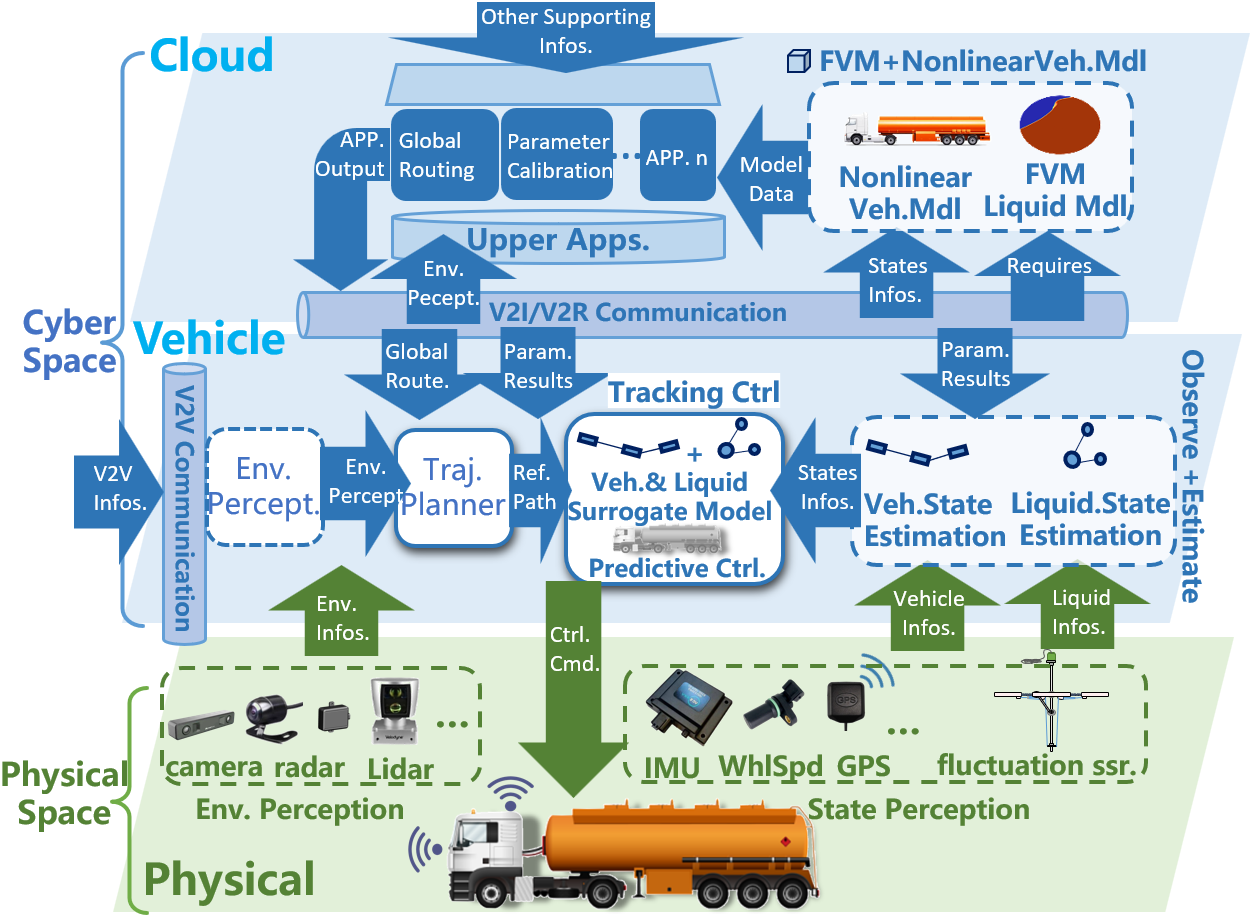
\includegraphics[width=3.5in]{fig/architecture1.png}
\vspace{-0.5cm}
\caption{Anti-rollover control scheme of this study.}
\label{fig:architecture}
\end{figure}
\vspace{-20pt}